\chapter{CloneRefactor}
CloneRefactor is the name of our clone detection and refactoring tool. It features the following novel functions:
\begin{itemize}
  \item Detection of clone classes rather than clone pairs.
  \item A novel detection method, aimed at extensibility.
  \item Detection of refactoring-oriented clone types, in addition to the literature clone types.
  \item Allows for automated refactoring of a subset of the detected duplication issues.
\end{itemize}
In this section we describe our approach and rationale for the design decisions regarding this tool.

\begin{figure}[H]
  \centering
  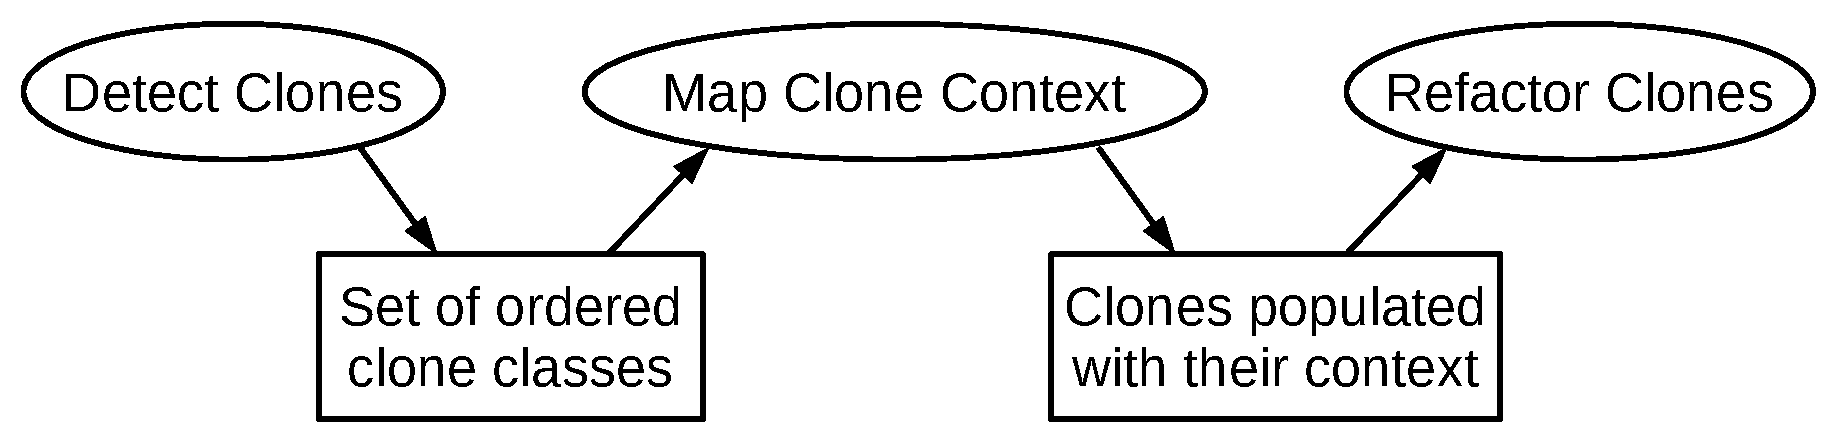
\includegraphics[width=0.8\columnwidth]{img/CloneRefactorOverall}
  \caption{CloneRefactor overall process.}
  \label{fig:clonerefactorprocess}
\end{figure}

Figure \ref{fig:clonerefactorprocess} shows the overall process used by CloneRefactor. First, we detect clones on basis of a Java codebase, given a Java project from disk and a configuration. The clone detection process is further explained in section \ref{sec:clonedetection}. After all clones are found, CloneRefactor maps the context of the clones. On basis of this context, CloneRefactor applies transformations to the source code for clones for which we have configured a refactoring.

\section{JavaParser}
A very important design decision for CloneRefactor is the usage of a library named JavaParser \cite{tomassetti2017javaparser}. JavaParser is a Java library which allows to parse Java source files to an abstract syntax tree (AST\footnote{An AST is a tree-representation of a source code file.}). JavaParser allows to modify this AST and write the result back to Java source code. This allows us to apply refactorings to the detected problems in the source code.

Integrated in JavaParser is a library named SymbolSolver. This library allows for the resolution of symbols using JavaParser. For instance, we can use it to trace references (methods, variables, types, etc) to their declarations (these referenced identifiers are also called ``symbols''). This is very useful for the detection of our refactoring-oriented clone types, as they make use of the fully qualified identifiers of symbols.

In order to be able to trace referenced identifiers SymbolSolver requires access to not only the analyzed Java projects, but also all its dependencies. This requires us to include all dependencies with the project. Along with this, SymbolSolver solves symbols in the JRE System Library (the standard libraries coming with every installation of Java) using the active Java Virtual Machine (JVM). This has a big impact on performance efficiency.

Because of the requirement of symbol resolution, the refactoring-oriented clone types are less suitable for large scale clone analysis.

\section{Clone Detection}\label{sec:clonedetection}
To detect clones, CloneRefactor parses the AST aqcuired from JavaParser to an unweighted graph structure. On basis of this graph structure, clones are detection. Dependent on the type of clones being detected, transformations may be applied. The way in which CloneRefactor was designed does not allow for several clone types to be detected simultaneously, in accordance with our clone type philosophy as described in chapter \ref{sec:unifying}.

The overall process regarding clone detection is displayed in figure \ref{fig:clonedetection}. First of all, we use JavaParser to read a project from disk and build an AST, one class file at a time. Each AST is then converted to a directed graph that maps relations between statements, further explained in section \ref{sec:clonegraph}. On basis of this graph, we detect clone classes and verify them using three thresholds (in order of importance):
\begin{itemize}
  \item Amount of tokens.
  \item Amount of statements.
  \item Amount of lines.
\end{itemize}
If the detection was configured to detect either type 2R, 3 or 3R clones we perform some type specific transformations on the resulting set of clones.

\begin{figure}[H]
  \centering
  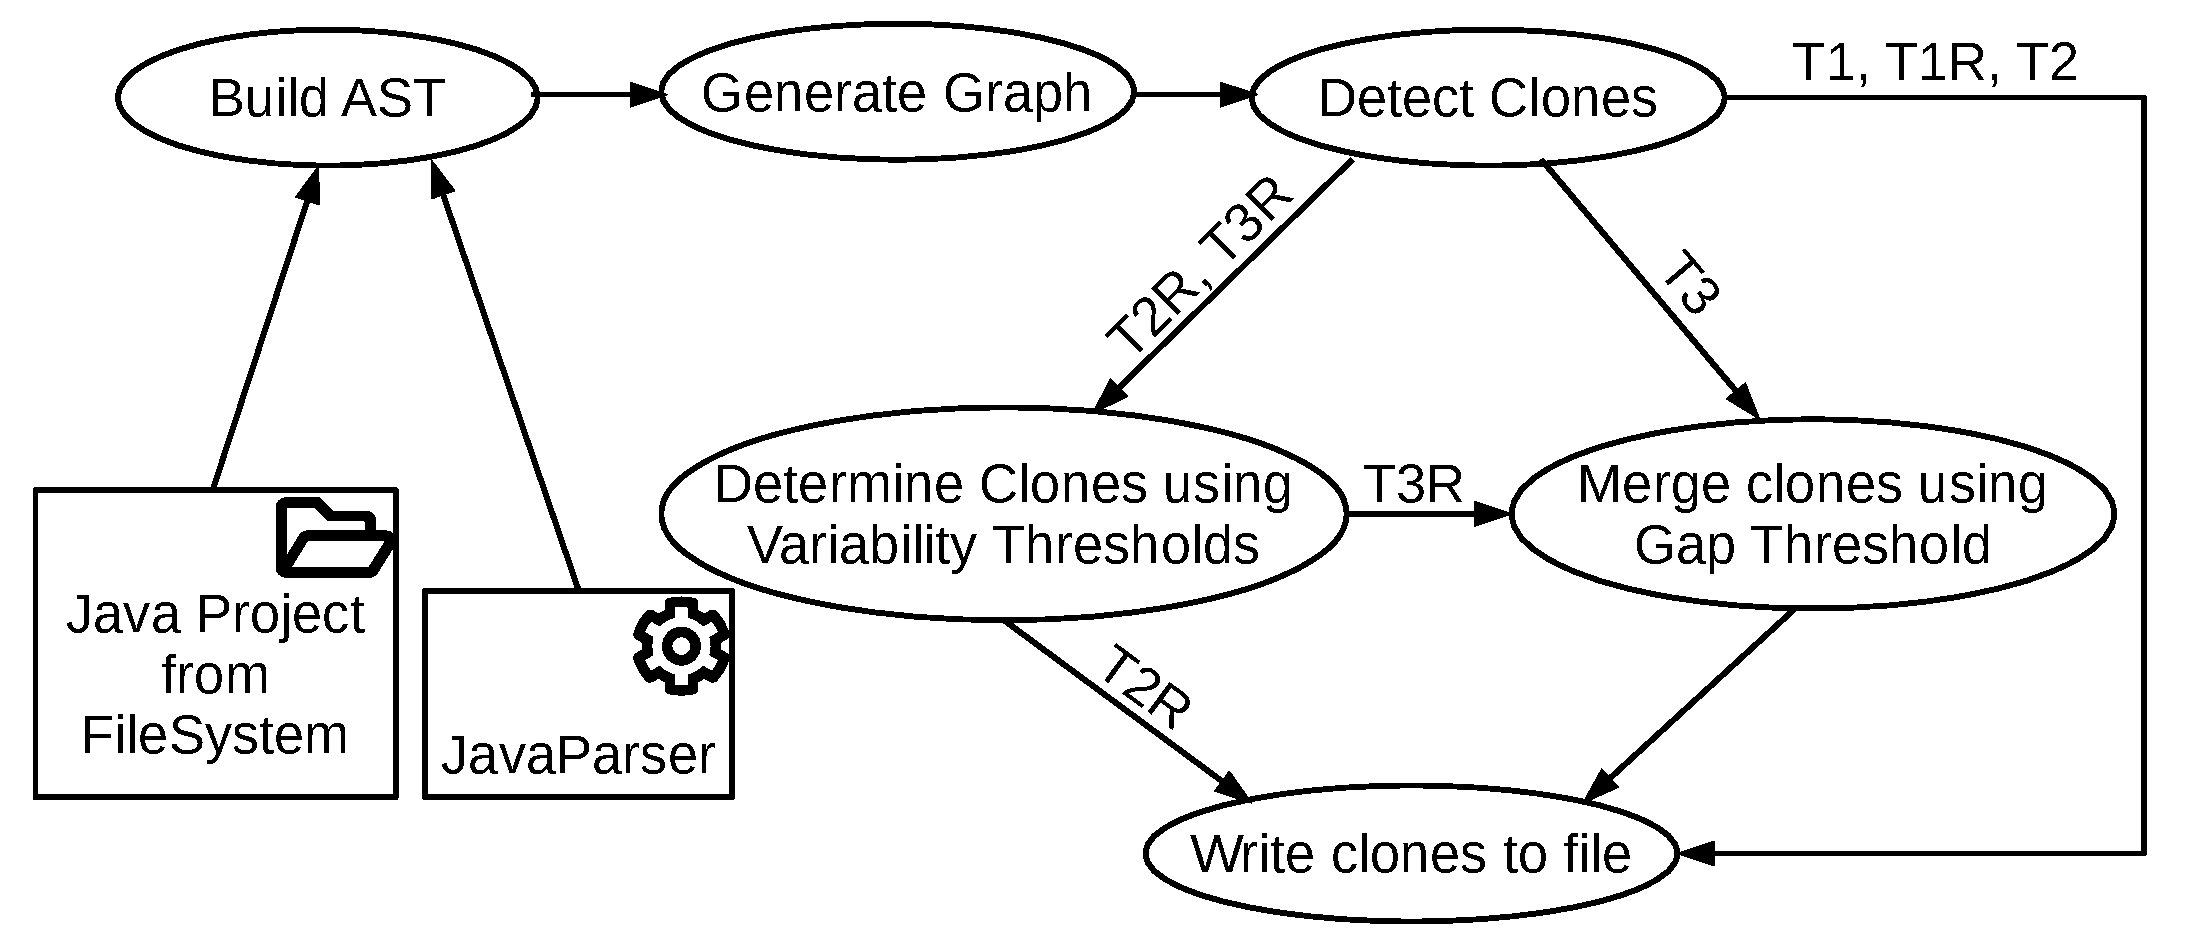
\includegraphics[width=1\columnwidth]{img/CloneDetection}
  \caption{CloneRefactor clone detection process.}
  \label{fig:clonedetection}
\end{figure}

\subsection{Generating the clone graph}\label{sec:clonegraph}
First of all, we parse the AST obtained from JavaParser into a directed graph structure. We have chosen to base our clone detection around statements as the smallest unit of comparison. This means that a single statement cloned with another single statement is the smallest clone we can find. The rationale for this lies in both simplicity and performance efficiency. This means we won't be able to find when a single expression matches another expression, or even a single token matching another token. This is in most cases not a problem, as expressions are often small and do not span the minimal size to be considered a clone in the first place (more about this in section \ref{sec:thresholds}).

\subsubsection{Filtering the AST}
As a first step towards building the clone graph, we preprocess the AST to decide which AST nodes should become part of the clone graph. We have decided to consider declarations and statements as the smallest compared entities. The main reasoning for this is because considering smaller AST constructs, like expressions, significantly increases the complexity and CPU usage of our clone detection and refactoring efforts.

Additionally, we exclude package declarations and import statements. These are omitted by most clone detection tools, as clones in import statements hold limited valuable information.

\subsubsection{Building the clone graph}\label{sec:buildingclonegraph}
Building the clone graph consists of walking the AST in-order for each declaration and statement. For each declaration/statement found, we map the following relations:
\begin{itemize}
  \item The declaration/statement preceding it.
  \item The declaration/statement following.
  \item The last \textbf{preceding} declaration/statement with which it is cloned.
\end{itemize}
We do not create a separate graph for each class file, so the statement/declaration preceding or following could be in a different file. While mapping these relations, we maintain a hashed map containing the last occurrence of each unique statement. This map is used to efficiently find out whether a statement is cloned with another. An example of such a graph is displayed in figure \ref{fig:clonegraphsimple}.

\begin{figure}[H]
  \centering
  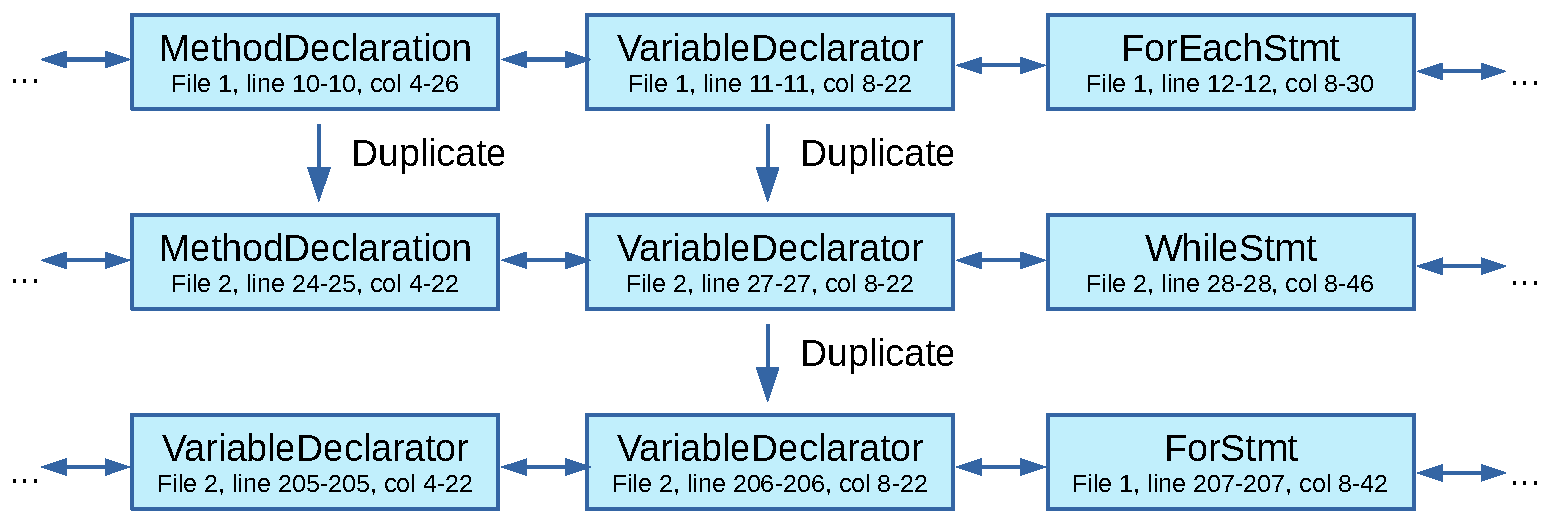
\includegraphics[width=1\columnwidth]{img/CodeGraph2}
  \caption{Abstract example of a part of a possible clone graph as built by CloneRefactor.}
  \label{fig:clonegraphsimple}
\end{figure}

We refer to the declarations and statements in this graph as \textit{nodes}. The relations \textit{next} and \textit{previous} in this graph are represented as an twodirectional arrow. The relations representing duplication are directed. This is a restriction we've chosen as it creates an important constraint for the clone detection process. This process is explained in section \ref{sec:detectingclones}.

\subsection{Comparing Statements/Declarations} \label{sec:comparingstuff}
In the previous section we described a ``duplicate'' relation between nodes in the clone graph built by CloneRefactor. Whether two nodes in this graph are duplicates of each other is dependent on the clone type. In this section, we will describe for each type how we compare statements and declarations to assess whether they are clones of each other.

CloneRefactor detects six different types of clones: T1, T2, T3, T1R, T2R and T3R. These types are further explained in chapter \ref{chap:clonetypes}. For \textbf{type 1} clones, CloneRefactor filters the tokens of a node to exclude its comments, whitespace and end of line (EOL) characters and then compares these tokens. For \textbf{type 2} clones, the tokens are further filtered to omit all identifiers and literals. \textbf{Type 3} clones do the same duplication comparison as type 2 clones.

For \textbf{type 1R} clones, this comparison is a lot more advanced. For \textit{method calls} we trace their declaration and use its fully qualified method signature for comparison with other nodes. For all \textit{referenced types} we trace their declarations and use assemble their fully qualified identifier for comparison with other nodes. For \textit{variables} we trace their declaration and their types. If the variable type is a primitive we can directly use it for comparison. If it is a referenced type, we have to trace this type first in order to collect their fully qualified identifier for comparison.

\textbf{Type 2R} clones allow any variation in literals, variables and method calls at this stage in the clone detection process. However, for \textit{literals} we do resolve their type in order to verify that they are of the same type. For \textit{variables} we also only verify that their types are the same (but not their names). For \textit{method calls}, we trace their declaration but only compare the fully qualified identifier for its return type and each of its arguments' types. Apart from that, we do not compare the names of method, class, interface and enum declarations.

In this stage, \textbf{type 3R} clones have the same compare rules as type 2R clones.

\subsection{Mapping graph nodes to code}
The clone graph, as explained in section \ref{sec:buildingclonegraph}, contains all declarations and statements in a source code. However, declarations and statements may themselves have child declarations and statements. To avoid redundant duplication checks, we exclude child declarations and statements from each node. Look at figure \ref{fig:clonegraph} for an example of how source code maps to AST nodes.

\begin{figure}[H]
  \centering
  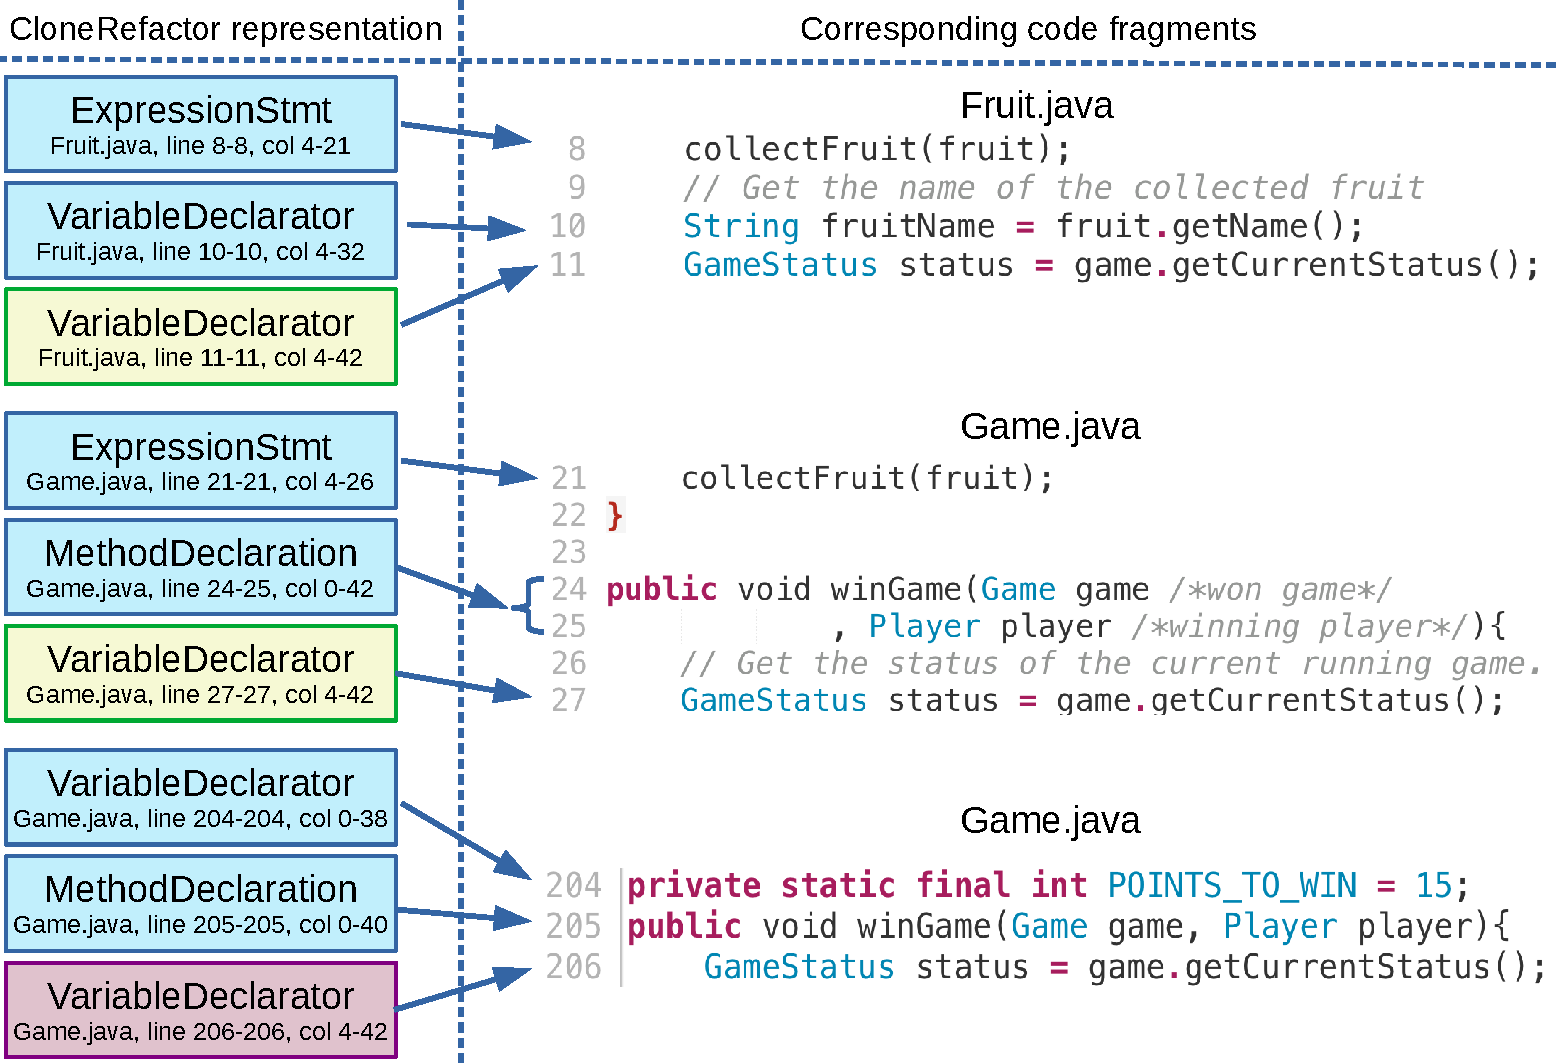
\includegraphics[width=1\columnwidth]{img/CloneGraphCode}
  \caption{CloneRefactor extracts statements and declarations from source code.}
  \label{fig:clonegraph}
\end{figure}

In line 24-25 of the code fragment, we see a \texttt{MethodDeclaration}. The node corresponding with this MethodDeclaration denotes all tokens found on these two lines, line 24 and 25. Although the statements following this method declaration (those that are part of its body) officially belong to the method declaration, they are not included in its graph node. Because of that, in this example, the \texttt{MethodDeclaration} on line 24-25 will be considered a clone of the \texttt{MethodDeclaration} on line 205 even though their bodies might differ. Even the range (the line and column that this node spans) does not include its child statements and declarations.

\subsection{Detecting Clones} \label{sec:detectingclones}
After building the clone clone graph, we use it to detect clones. We decided to focus on the detection of clone classes rather than clone pairs because clone pairs do not provide a general overview of all entities containing the clones, with all their related issues and characteristics \cite{fontana2012duplicated}. Although clone classes are harder to manage, they provide all information needed to plan a suitable refactoring strategy, since this way all instances of a clone are considered. Another issue that results from grouping clones by pairs: clone reference amount increases according to the binomial coefficient formula (two clones form a pair, three clones form three pairs, four clones form six pairs, and so on), which causes a heavy information redundancy \cite{fontana2012duplicated}.

As stated in the previous section, nodes in the graph link to \textit{preceding} cloned statement. This implies that the first node that is cloned does not have any clone relation, as there are no clones preceding it (only following it). Because of this, we start our clone detection process at the final location encountered while building the graph. For this node, we collect all nodes it is cloned with. Even though the final node only links to the preceding node it is cloned with, we can collect all clones. This is because the preceding clone also has a preceding clone (if applicable) and we can follow this trail to collect all clones of a single node. As an example, we convert the code example shown in figure \ref{fig:clonegraph} to a clone graph as displayed in figure \ref{fig:clonegraph2}.

\begin{figure}[H]
  \centering
  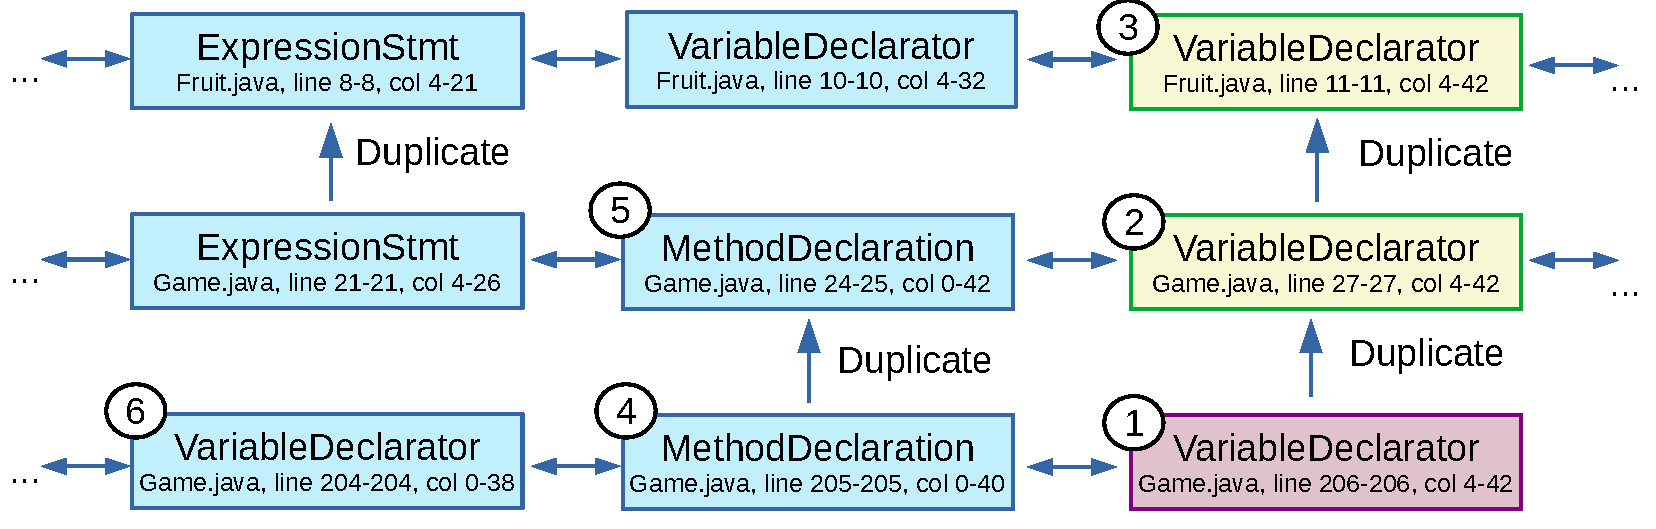
\includegraphics[width=1\columnwidth]{img/CodeGraphExample}
  \caption{Example of a clone graph built by CloneRefactor.}
  \label{fig:clonegraph2}
\end{figure}

Using the example shown in figure \ref{fig:clonegraph} and \ref{fig:clonegraph2} we can explain how we detect clones on basis of this graph. Suppose we are finding clones for two files and the final node of the second file is a variable declarator. This final node is represented in the example figure by the purple box (1). We then follow all ``duplicate'' relations until we have found all clones of this node (2 and 3). We now have a single statement clone class of three clone instances (1, 2 and 3).

Next, we move to the previous line (4). Here again, we collect all duplicates of this node (4 and 5). For each of these duplicates, we check whether the node following it is already in the clone class we collected in the previous iteration. In this case, (2) follows (5) and (1) follows (4). This means that node (3) does not form a `chain' with other cloned statements. Because of this, the clone class of (1, 2 and 3) comes to an end. It will be checked against the thresholds, and if adhering to the thresholds, considered a clone.

We then go further to the previous node (6). In this case, this node does not have any clones. This means we check the (2 and 5, 1 and 4) clone class against the thresholds, and if it adheres, consider it a clone. Dependent on the thresholds, this example can result in a total of two clone classes.

Eventually, following only the ``previous node'' relations, we can get from (6) to (2). When we are at that point, we will find only one cloned node for (2), namely (3). However, after we check this clone against the thresholds, we check whether it is a subset of any exisiting clone. If this is the case (which it is for this example), we discard the clone.

\subsubsection{Removing redundant clone classes}\label{sec:conceptualremovingredundant}
The clone detection method used by CloneRefactor can, for various reasons,%Should I list these? Listing them could be a section on its own, as I'd have to show examples to make it concrete.
result in redundant clone classes. After the insertion of each newly detected clone, we check whether it is redundant and/or any of the existent clones has become redundant by adding this clone. A clone is redundant if it is a subset of an existing clone. We define the subset relation between clones as follows:

\begin{equation}\label{eq:subset}
C_1 \subseteq C_2 \Leftrightarrow \forall (i_1 \in C_1) \text{ } \exists (i_2 \in C_2) \text{ } F i_1 = F i_2 \wedge R i_1 \subseteq R i_2
\end{equation}

Where \textit{C} refers to a clone class (a set of clone instances), \textit{i} refers to a clone instance, \textit{F} is the file in which a clone instance is located and \textit{R} is the range of tokens that a clone instance spans. For each clone added, we remove all existing clones that are a subset of the newly added clone:

\begin{equation}\label{eq:removeall}
S = S \setminus \{C_{existing} \subseteq C_{new}\text{ }|\text{ }C_{existing} \in S\}
\end{equation}

Where \textit{S} is the set of all clone classes that are found up in until this point. Likewise, we should not add the new clone to our list of clones if its a subset of an existing clone. Because of that, we check for each clone added whether there exists a clone of which the newly added clone is a subset:

\begin{equation}\label{eq:removeexisting}
\{C_{existing} \subseteq C_{new}\text{ }|\text{ }C_{existing} \in S\} = \emptyset \Rightarrow S = S \cup C_{new}
\end{equation}

If the newly added clone is a subset of an existing clone, we do not add it to the set of clone classes. This way we avoid redundant clone classes being detected by CloneRefactor.

\subsection{Validating the type 2R variability threshold}
In the definition of type 2R clones (see section \ref{sec:type2r}) we described how type 2R clones work on basis of a variability threshold. This threshold, shown more formally in formula \ref{eq:type2r}, is checked by CloneRefactor. Implementing such a threshold involves some important design decisions, and has a lot of underwater complexity. In this section we explain how CloneRefactor detects type 2R clones on basis of this variability threshold. This process is done as a postprocessing step after clone detection. The type 2R clone detection process is described in more detail in section \ref{sec:comparingstuff}. In short, this process detects clones allowing for any variability between expressions. This postprocessing step then determines which (parts of) these clones are valid by the configure variability threshold.

\begin{figure}[H]
  \centering
  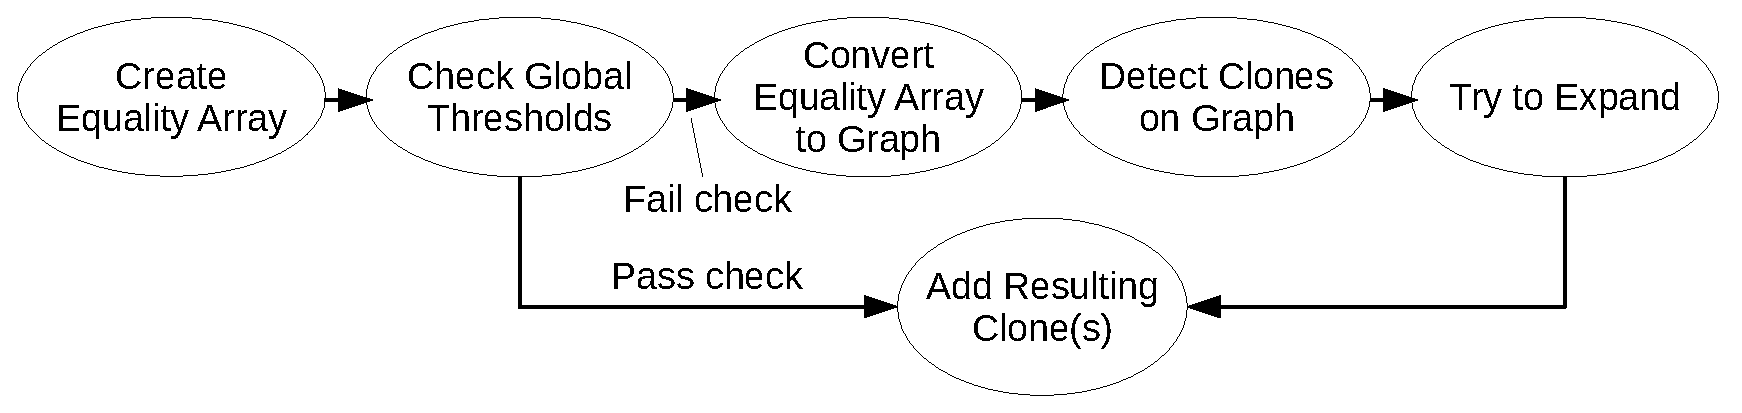
\includegraphics[width=1\columnwidth]{img/CloneRefactorT2RFlow}
  \caption{Process used to check the variability threshold for T2R clones.}
  \label{fig:clonerefactort2rflow}
\end{figure}

Figure \ref{fig:clonerefactort2rflow} shows the steps that CloneRefactor performs to find clones conforming with the type 2R variability threshold. Each of the following paragraphs will explain a step from this figure.

\subsubsection{Create equality array}
To determine the difference in literals, method calls and variables, we convert the code to an equality array. This equality array converts each (group of) token(s) to a number unique to that (group of) tokens. Each literal, method call or variable becomes a positive number, whereas each other token becomes a negative number. An example of two code fragments converted to equality arrays is displayed in figure \ref{fig:equalityarrays}.

\begin{figure}[H]
  \centering
  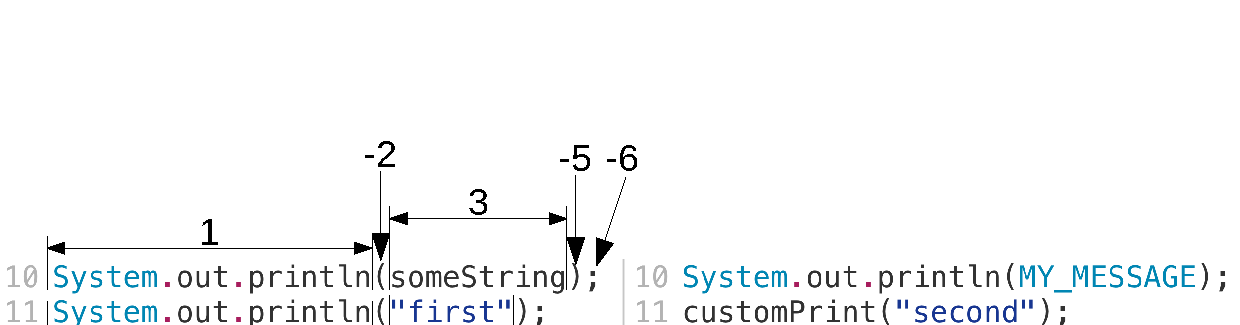
\includegraphics[width=1\columnwidth]{img/equality}
  \caption{The conversion of code to an equality array.}
  \label{fig:equalityarrays}
\end{figure}

The equality array for each of the lines in this example is shown in table \ref{table:equalityarrays}.

\begin{table}[H]
\begin{center}
 \caption{The equality arrays in our example figure \ref{fig:equalityarrays}.} \label{table:equalityarrays}
 \medskip
\begin{tabular}{|l|l|l|}
\hline
Node (n) & Equality Array (E) \\ \hline
1        & {[}1, -2, 3, -5, -6{]} \\ \hline
2        & {[}1, -2, 7, -5, -6{]} \\ \hline
3        & {[}1, -2, 4, -5, -6{]} \\ \hline
4        & {[}8, -2, 9, -5, -6{]} \\ \hline
\end{tabular}
\end{center}
\end{table}

In the example of figure \ref{fig:equalityarrays} the fragment on the left (consisting of $n_1$ and $n_2$) and the fragment on the right (consisting of $n_3$ and $n_4$) are two clone instances of a clone class. Table \ref{table:equalityarrays} shows their corresponding equality arrays.

\subsubsection{Checking global thresholds}
Using the equality arrays explained in the previous section, we can determine the variability threshold of any clone class. We calculate the variability of the example given in table \ref{table:equalityarrays} as follows:

\begin{equation}\label{eq:variabilityclonerefactor}
\frac{|\{x>0 \land y>0 \land x \neq y\text{ }|\text{ }x \in E_1 \cup E_2, y \in E_3 \cup E_4\}|}{(|E_1|+|E_2|)+(|E_3|+|E_4|)}*100
\end{equation}

Where \textit{E} refers to the equality arrays shown in table \ref{table:equalityarrays}. When we apply this equation to the example clone classes displayed in figure \ref{fig:equalityarrays}, we get the following sum:

\begin{equation}\label{eq:sumequality}
\frac{|{(3,4), (1,8), (7,9)}|}{(5+5)+(5+5)}*100 = \frac{3}{20}*100 = 15\%
\end{equation}

So for the example given in figure \ref{fig:equalityarrays} we have a variability of 15\%. In CloneRefactor, the maximum variability percentage is a threshold that is entered in a configuration file. If a clone adheres to this threshold, it will stay in the set of found clones. However, if it does not adhere to the thresholds, a problem arises. Because a clone does not adhere to the thresholds, it does not yet mean it has to be discarded. This is because an invalid clone class can still contain valid clones that are a subset of the invalid clone (our definition of subsets of clones is given in section \ref{sec:conceptualremovingredundant}).

%Two nodes are considered clones of each other if the size of their equality array is equal and all negative numbers in the equality array are equal.


When a found clone class does not adhere to the global thresholds as explained in the previous section, we need to determine whether it contains any valid subclones. Below, we explain a few cases of valid subclones that may exist within an invalid clone class.

\begin{figure}[H]
\begin{parcolumns}{2}
\colchunk[1]{
\begin{javacode}
doA(a, b, c);
|\highlightYellow|doA();
|\highlightYellow|doB();
|\highlightYellow|doC();
\end{javacode}}
\colchunk[2]{
\begin{javacode}
doB(d, e, f);
|\highlightYellow|doA();
|\highlightYellow|doB();
|\highlightYellow|doC();
\end{javacode}}
\end{parcolumns}
\caption{One node in a type 2R clone has a high variability.}
\label{fig:2rvariabilityhigh1}
\end{figure}

The first line of the cloned fragment shown in figure \ref{fig:2rvariabilityhigh1} has a high variability with its cloned fragement. However, the rest of this method does not have any variability. The global thresholds could indicate a too high variability and thus render this clone invalid. However, in this case, it might still have a valid subclone.

\begin{figure}[H]
\begin{parcolumns}{3}
\colchunk[1]{
\begin{javacode}
|\highlightYellow|doA();
|\highlightYellow|doB();
|\highlightYellow|doC();
\end{javacode}}
\colchunk[2]{
\begin{javacode}
|\highlightYellow|doA();
|\highlightYellow|doB();
|\highlightYellow|doC();
\end{javacode}}
\colchunk[3]{
\begin{javacode}
doD();
doE();
doF();
\end{javacode}}
\end{parcolumns}
\caption{One clone instance in a type 2R clone has a high variability.}
\label{fig:2rvariabilityhigh2}
\end{figure}

Another example of high variability between clones, in which a valid subclone can be found, is displayed in figure \ref{fig:2rvariabilityhigh2}. In this case, one clone instance has such a high variability that it shouldn't be refactored. In this case, the clone instance with high variability should be removed.

\begin{figure}[H]
\begin{parcolumns}{3}
\colchunk[1]{
\begin{javacode}
|\highlightYellow|doA();
|\highlightYellow|doB();
doC();
doC();
\end{javacode}}
\colchunk[2]{
\begin{javacode}
doD();
|\highlightYellow|doA();
|\highlightYellow|doB();
doD();
\end{javacode}}
\colchunk[3]{
\begin{javacode}
doE();
doE();
|\highlightYellow|doA();
|\highlightYellow|doB();
\end{javacode}}
\end{parcolumns}
\caption{A small subset of nodes has a high variability.}
\label{fig:2rvariabilityhigh3}
\end{figure}

Figure \ref{fig:2rvariabilityhigh3} shows an example of a clone class where the valid sequence inside the clone does not align.

If the check for global thresholds fails, we have to seek for valid clones within the clone class. In a single invalid clone class can be zero to many subclones. This requires an extensive search for such clones. This problem is very related to the problem of clone detection, except now it is within the boundaries of a single clone class except for an entire codebase. Because of that, just like the clone detection process, we build a clone graph and detect clones on it. This process is explained over the following sections.

\subsubsection{Convert Equality Array to Graph}
After the global threshold check has failed, we build a clone graph on basis of the equality arrays.

\begin{figure}[H]
\begin{parcolumns}{3}
\colchunk[1]{
\begin{javacode}
|\highlightYellow|doA(); //{1, -2}
|\highlightYellow|doB(); //{3, -2}
doC(); //{4, -2}
doC(); //{4, -2}
\end{javacode}}
\colchunk[2]{
\begin{javacode}
doD(); //{5, -2}
|\highlightYellow|doA(); //{1, -2}
|\highlightYellow|doB(); //{3, -2}
doD(); //{5, -2}
\end{javacode}}
\colchunk[3]{
\begin{javacode}
doE(); //{6, -2}
doE(); //{6, -2}
|\highlightYellow|doA(); //{1, -2}
|\highlightYellow|doB(); //{3, -2}
\end{javacode}}
\end{parcolumns}
\caption{Cloned code fragments from figure \ref{fig:2rvariabilityhigh3} together with their equality arrays.}
\label{fig:2rvariabilityhigh4}
\end{figure}

In figure \ref{fig:2rvariabilityhigh4} we display the equality arrays for each of the lines of a code example with a complex distribution of cloned fragments. We can convert this to a graph, using a similar process as the graph creation process used for clone detection. In this case, duplicate relations represent nodes of which their equality arrays are within the variability threshold. In figure \ref{fig:2rvariabilityhigh4} all relations are between equal equality arrays, but this does not always have to be the case. Large equality arrays, denoting statements that consist of many tokens, may have some variability and still be considered duplicates in this graph.

\begin{figure}[H]
  \centering
  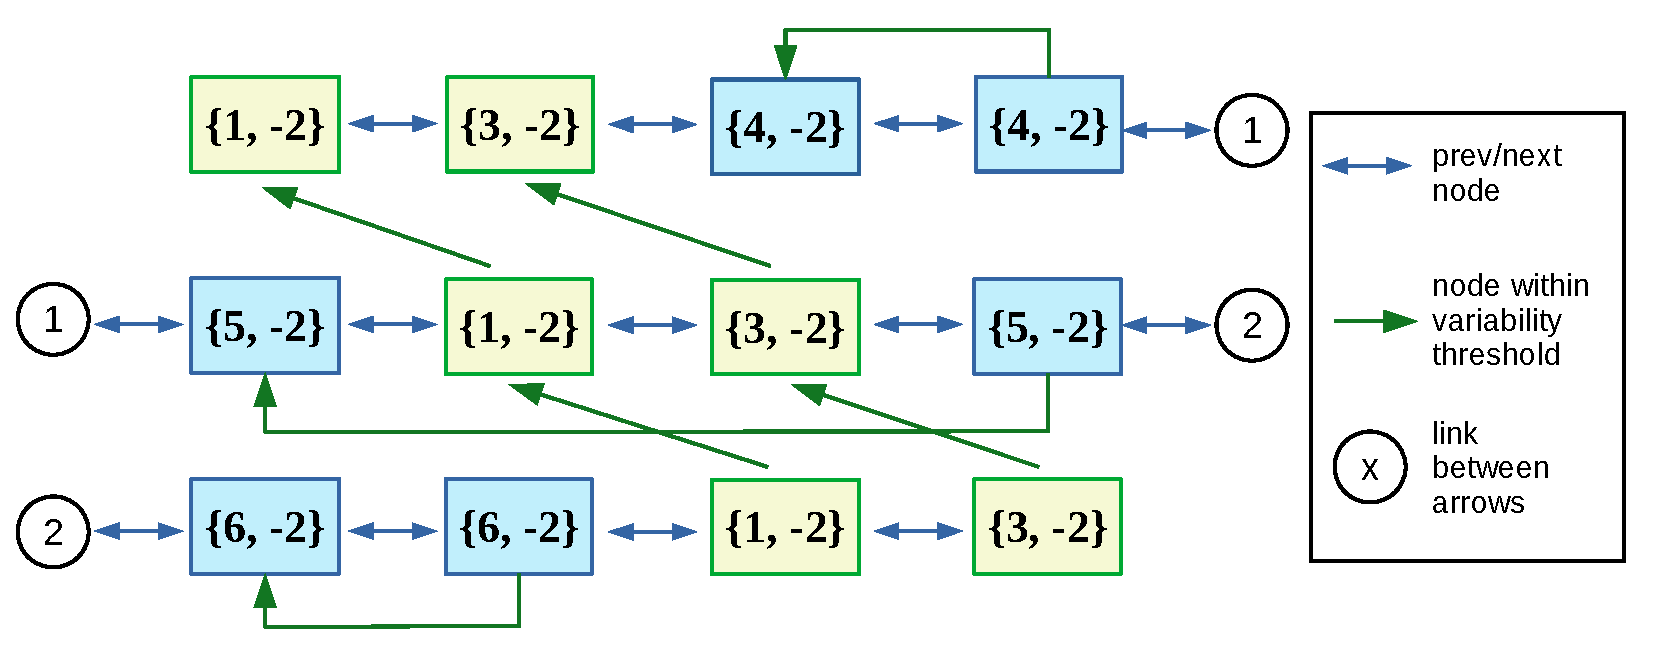
\includegraphics[width=1\columnwidth]{img/T2RGraph}
  \caption{Graph representation of the code example displayed in figure \ref{fig:2rvariabilityhigh4}.}
  \label{fig:clonerefactorprocess}
\end{figure}


\subsubsection{Detect Clones on Graph}
\todo{TODO}
\begin{equation}\label{eq:t2rcloneequality}
E_1\text{ is cloned with }E_2\text{ iff }|E_1|=|E_2| \land \forall (x \in E_1) \exists (y \in E_2) x<0 \lor y<0 \Rightarrow x=y
\end{equation}

\subsubsection{Try to Expand}
\todo{TODO}

\subsection{Checking for type 3 opportunities}
\todo{TODO}
